\section{Arista}

\subsection{Introduction}

Arista Networks is an industry leader and present in many financial organizations, enterprises, and Fortune 500 companies. It is heavily used by carriers and organizations with demanding networks. 

While there is no Arista equipment in Rubin's network, some of the partners of the LHN have many Arista deployments and posees extensive experience on it. 

The quotations have been made by an Arista partner, and can be found in the following link <insert link>

\subsection{Hardware}

The hardware offered by the vendor is the \href{https://www.arista.com/assets/data/pdf/Datasheets/7260X3_Datasheet.pdf}{7260X3-64}, some of its features are:
\begin{itemize}
    \item 64 x QSFP100 (support for 10G or 100G)
    \item 2RU
    \item Up to 12.8 terabits per second
    \item Latency from 450ns
\end{itemize}

\begin{figure}
    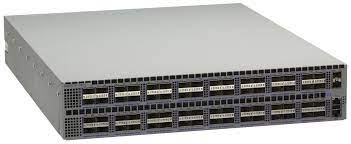
\includegraphics[width=11cm]{images/arista_7260X3-64.jpg}
    \centering
    \caption{Arista 7260X3-64}
  \end{figure}

\subsection{License}

The provided license is the version E which is perpetual for the use of the product at a fixed price. Some of its features licensed:

\begin{itemize}
  \item Dynamic Routing (OSPF, BGP, etc)
  \item PIM (SM,BSR,MBR)
  \item Anycast RP
  \item VXLAN Bridging + Routing
  \item GRE Tunnels
  \item Network Address Translation
  \item Base Licensing (L2,MLAG,VRFs,QOS,Linux tools and services, etc)
\end{itemize}

Details of the license can be found \href{https://www.arista.com/en/support/product-documentation/eos-feature-licensing}{here.}


\subsection{Network Design}
\subsection{Support}

Vendor has included support for 5 years with the following features:
\begin{itemize}
  \item Hardware replacement NBD
  \item Access to Arista TAC 24/7 through customer portal with capacity of unlimited users
  \item Software downloads
\end{itemize}

Details of A-Care support from Arista can be found \href{https://www.arista.com/assets/data/pdf/A-CareServicesOverview.pdf}{here.}

\subsection{Training}

Vendor provides free training and virtual labs with selfpaced modules. There are also certification paths with instructor led training with different costs depending on the complexity.

Details of training offerings can be found \href{https://www.arista.com/en/support/hands-on-training}{here.}

\subsection{Pros/Cons}

\subsubsection{Pros}
\begin{itemize}
  \item The vendor has deep expertise and solid products to meet the needs of large and/or advanced enterprises, including cloud providers and financial services.
  \item Arista has a strong support capabilities, it is one of few vendors that doesn't outsource technical support.
  \item Arista had only 14 CVE reports since 2015. That's considerably lower than the other vendors. 
  \item Rubin's partners in the long haul network have plenty of experience with Arista equipment, becoming a good resource of information and help for Rubin's engineers. 
  \item The CLI of Arista EOS is very similar to Cisco CLI, hence the previous experience of Rubin's engineers with Cisco will help to adapt to Arista environment.
  \item Arista supports all open standards required by Rubin's network design.
  \item License provided is for the lifetime of the product.
\end{itemize}

\subsubsection{Cons}
\begin{itemize}
  \item Arista has limited channel and sales resources outside North America, however, there is a depot in Chile capable of shipping parts. 
  \item The Puppet modules of Arista are not updated, however its Ansible modules are still being developed and constantly updated. 
  \item There's no experience in Rubin with Aristas equipment
\end{itemize}

\subsection{Closing Comments}

Arista provides hardware with good performance running on a reliable operating system. It is priced competitively and the perpetual license is a welcome feature. 

The support and involvement provided the pre-sales Arista team it is above our expectations and there's interest from the provider to work with Rubin. 

The similarities of the CLI to the Cisco CLI makes it easier for Rubin's engineers to learn and understand the components of the operating system. 

The capability to open a shell session in the underlaying Linux system allows to perform further troubleshooting not available on Cisco devices. All Rubin's engineers are quite proficient in Linux hence accessing its tools in network devices is very appreciated. 

The low amount of CVEs reported proves that the software is of good quality and also implies that emergency patches with potential outages is not a common event. 